\begin{frame}

    \begin{center}
        \Huge Part III: Monotone Computations
    \end{center}
    
\end{frame}

\begin{frame}{Flow formulas}
    \begin{minipage}{0.5 \linewidth}
        \tikzstyle{undir} = [thick]
\tikzstyle{dir} = [thick, ->, bend left = 10]
\tikzstyle{ver} = [thick, ->, draw, circle]

\begin{tikzpicture}[black, >=latex]
    \node[ver] (A) at (0, 0) {};
    \node[ver] (B) at (1.9, 1.9) {};
    \node[ver] (C) at (3, 0) {};
    \node[ver] (D) at (4, 1.2) {};
    \node[ver] (E) at (3.3, 3.7) {};
    \node[ver] (F) at (-0.5, 3) {};
    \node at (0, -0.2) {};

    \only<1>{
        \draw[undir] (A) to (B);
        \draw[undir] (A) to (C);
        \draw[undir] (B) to (C);
        \draw[undir] (C) to (D);
        \draw[undir] (B) to (D);
        \draw[undir] (D) to (E);
        \draw[undir] (E) to (F);
        \draw[undir] (F) to (A);
        \draw[undir] (B) to (F);
    }
    
	\only<2->{
        \draw[dir] (A) to (B);
        \draw[dir] (A) to (C);
        \draw[dir] (B) to (C);
        \draw[dir] (C) to (D);
        \draw[dir] (B) to (D);
        \draw[dir] (D) to (E);
        \draw[dir] (E) to (F);
        \draw[dir] (F) to (A);
        \draw[dir] (B) to (F);

        \draw[dir] (B) to (A);
        \draw[dir] (C) to (A);
        \draw[dir] (C) to (B);
        \draw[dir] (D) to (C);
        \draw[dir] (D) to (B);
        \draw[dir] (E) to (D);
        \draw[dir] (F) to (E);
        \draw[dir] (A) to (F);
        \draw[dir] (F) to (B);
    }
\end{tikzpicture}

        \putpos{15}{100}{\includegraphics[scale = 0.1]{pics/utia-duck.png}}
    \end{minipage}%
    \begin{minipage}{0.5 \linewidth}
        \pause
        \pause
        \begin{itemize}
            \item $v\colon ~ \sum\limits_{e \in E^{\mathrm{in}}_v} x_{e} -
                \sum\limits_{e \in E^{\mathrm{out}}_v} x_{e} = c(v)$ 
                \textcolor{red}{$(\mathbb{R})$};
            \item $\sum\limits_{v} c(v) = 1$ \textcolor{red}{$(\mathbb{R})$};
            \item graph degree: $d$.
        \end{itemize}
    \end{minipage}

    \pause
    \vspace{0.2cm}
    \begin{itemize}
        \item{} There is an efficient Nullstellensatz proof of $\Flow$.
        \item{} [Alekhnovich, Razborov 03] If $G$ is an expander $\Rightarrow$ any
            resolution proof has size $2^{\Omega(n)}$.
    \end{itemize}

    \pause

    \begin{corollary}[G\"{o}\"{o}s, Kamath, Robere, S 19]
        There is a monotone function in $\NC^2$ that cannot be computed by subexponential monotone
        circuits.
    \end{corollary}

\end{frame}



\begin{frame}{Monotone Computations}

    \begin{minipage}{0.33\linewidth}
        \centering
        Formulas
        \vspace{0.2cm}
        
        \input{pics/mon-form.tex}
    \end{minipage}
    \begin{minipage}{0.33\linewidth}
        \centering
        Circuits
        \vspace{0.2cm}
        
        \begin{tikzpicture}[>=latex]
    \node[circle, minimum size = 0.5cm, inner sep = 0pt, draw, fill = LEIorange!5] (a) at (5, 2)
        {$x$};
    \node[circle, minimum size = 0.5cm, inner sep = 0pt, draw, fill = LEIorange!5] (b) at (3.5, 2)
        {$y$};
    \node[circle, minimum size = 0.5cm, inner sep = 0pt, draw, fill = LEIorange!5] (c) at (4.5, 1)
        {$\lor$};
    \node[circle, minimum size = 0.5cm, inner sep = 0pt, draw, fill = LEIorange!5] (d) at (2.7, 1)
        {$z$};
    \node[circle, minimum size = 0.5cm, inner sep = 0pt, draw, fill = LEIorange!5] (e) at (3.8, 0.3)
        {$\land$};
    %\node[circle, minimum size = 0.5cm, inner sep = 0pt, draw, fill = LEIorange!5] (f) at (5.2, 0.6)
     %   {$y$};
    \node[circle, minimum size = 0.5cm, inner sep = 0pt, draw, fill = LEIorange!5] (g) at (4, -0.5)
        {$\lor$};

    \draw[->] (a) -- (c);
    \draw[->] (b) -- (c);
    \draw[->] (c) -- (e);
    \draw[->] (d) -- (e);
    \draw[->] (e) -- (g);
    \draw[->] (c) -- (g);
    \draw[->] (g) -- ++(0, -0.5);
\end{tikzpicture}
    \end{minipage}
    \begin{minipage}{0.32\linewidth}
        \centering
        More circuits
        \vspace{0.2cm}
        
        \input{pics/mon-r-ckt.tex}
    \end{minipage}

    \pause
    Why do we care about lower bounds on monotone computations?
    \begin{itemize}
        \item We can proof something!
            \pause
        \item We can control relative error.
            \pause
        \item Strong enough lower bounds on monotone circuits $\Rightarrow$ lower bounds on general
            circuits.
            \pause
        \item Secret sharing/cryptography.
    \end{itemize}
\end{frame}


\begin{frame}{Communication Protocols. $f\colon U \times V \to T$}
    \begin{center}
    	\onslide<1->{
    \tikzstyle{op1} = [opacity = 0]
    \tikzstyle{op2} = [opacity = 0]
    \tikzstyle{op3} = [opacity = 0]
    \tikzstyle{op4} = [opacity = 0]
}
\only<2->{\tikzstyle{op2} = [opacity = 1]}
\only<3->{\tikzstyle{op3} = [opacity = 1]}
\only<4->{\tikzstyle{op4} = [opacity = 1]}

\begin{tikzpicture}[>=latex]
    \node (alice) at (0, 0) {\includegraphics[scale = 0.15]{pics/utia-food-1.png}};
    \node (bob) at (7, 0) {\includegraphics[scale = 0.15]{pics/utia-food-2.png}};
    \node[above = 0.3 of alice] {$x \in U$};
    \node[above = 0.3 of bob] {$y \in V$};

    \path (alice.east) -- (bob.west) node[midway, above = 2.3] {\Large $f(x, y) = ?$};
    \draw[op2, ->, thick] ($(alice.east) + (0.3, 1)$) -- ($(bob.west) + (-0.3, 1)$) node[midway, above]
        {$r_1 = a(x)$};
    \draw[op3, <-, thick] ($(alice.east) + (0.3, 0.2)$) -- ($(bob.west) + (-0.3, 0.2)$)
        node[midway, above] {$r_2 = b(y, r_1)$};
    \draw[op4, ->, thick] ($(alice.east) + (0.3, -0.2)$) -- ($(bob.west) + (-0.3, -0.2)$);
    \draw[op4, ->, thick] ($(alice.east) + (0.3, -0.6)$) -- ($(bob.west) + (-0.3, -0.6)$)
        node[midway, below] {$\vdots$}; 
\end{tikzpicture}    
    \end{center}

    \pause
    \pause
    \pause
	\pause

    \begin{itemize}
        \item Depth is the number of rounds (in the worst case).
        \item Size is the number of possible configurations.
    \end{itemize}
\end{frame}


\begin{frame}{$\KW$ Relation [Karchmer, Wigderson 90]}
    Let $U, V \subseteq \{0, 1\}^{n}$ and $U \cap V = \emptyset$.

    \vspace{0.1cm}
    $\KW$:
    \begin{itemize}
        \item Alice gets $u \in U$, Bob gets $v \in V$;
        \item goal: find $i$ such that $u_i \neq v_i$.
    \end{itemize}
    \pause
    Monotone version $\KWm$:
    \begin{itemize}
        \item goal: find $i$ such that $u_i = 1 \land v_i = 0$.
    \end{itemize}

    \pause

    \begin{theorem}[Karchmer, Wigderson 90]
        \alert{Monotone} formula for a function $f$ of size $S$ $\Leftrightarrow$ communication protocol
        for \alert{$\KWm$} $\KW$ of size $S$, where $U \coloneqq f^{-1}(1), V \coloneqq f^{-1}(0)$.
    \end{theorem}
\end{frame}


\begin{frame}{$\KWm$ is a ``Complete Relation''}

    \begin{itemize}
        \item $\mathcal{S} \subseteq U \times V \times \mathcal{O}$;
        \item define $F_{\mathcal{S}}\colon \{0, 1\}^m \to \{0, 1\}$ such that
            $\DCC(\KWm[F_{\mathcal{S}}]) = \DCC(S)$.
    \end{itemize}

    \pause

    \vspace{-0.2cm}
    \begin{center}
        \tikzstyle{ops} = [alt=<{#1}>{opacity = 1}{opacity = 0}]

\begin{tikzpicture}
    \draw[thick, rounded corners = 2pt] (0, 0) rectangle (4, 3);
    \node at (-1, 1.5) {$Y \coloneqq \{0, 1\}^{n k}$};
    \node at (5, 1.5) {};
    \node at (2, 3.3) {$Z \coloneqq \{0, 1\}^{n \ell}$};

    \draw[red!30, fill = red!10, rounded corners = 3pt] (0.3, 0.1) rectangle (1, 2.9)
        node[midway, red!80] {$D_1$};
    \draw[green!50!black, fill = green!30, rounded corners = 3pt, opacity = 0.5] (0.5, 0.4) rectangle
        (3.5, 0.9) node[midway, green!20!black] {$D_2$};
    \draw[blue!50!black, fill = blue!30, rounded corners = 3pt, opacity = 0.5] (0.7, 2) rectangle
        (3.4, 2.85) node[midway, blue!20!black] {$D_3$};
    \draw[ops = 6, very thick, red] (-1, 0.5) -- (5, 0.5);
    \draw[ops = 7, very thick, red] (3, -0.5) -- (3, 3.5);
\end{tikzpicture}
    \end{center}

    \pause
    $F_{\mathcal{S}}(1, 1, 0, \dots) \coloneqq 1$\pause, ~~~$F_{\mathcal{S}}(1, 0, 0, \dots) \coloneqq 0$

    \pause
    \begin{lemma}
        $\DCC(\KWm[F_{\mathcal{S}}]) = \DCC(S)$.
    \end{lemma}

    \pause
    \putpos{250}{110}{\includegraphics[scale = 0.1]{pics/utia-think.png}}

\end{frame}

\begin{frame}{$\Search_{\varphi}$ [Lov{\'{a}}sz, Naor, Newman, Wigderson et al. 94]}
    
    $\varphi(z) \coloneqq \bigwedge\limits_{i = 1}^{m} C_i$ is unsatisfiable CNF formula.
    \pause
    
    $\Search_{\varphi} \subseteq \{0, 1\}^n \times [m]$:
    \begin{itemize}
        \item $(\alpha, i) \in \Search_{\varphi} \Leftrightarrow C_{i}(\alpha) = 0.$
    \end{itemize}

    \pause
    \vspace{0.1cm}
    Communication version:
    \begin{itemize}
        \item ``gadget'' $g\colon X \times Y \to \{0, 1\}$;
    \end{itemize}

    \pause
    \begin{center}
        \begin{tikzpicture}
    \node[thick, circle, draw] (S) at (0, 0) {\Large $S$};
    
    \foreach \i in {1, 2, ..., 5}{
        \node (z\i) at (-3 + \i, -1.5) {$z_{\i}$};
        \draw[->] (z\i) -- (S);
    }
    
    \node[minimum height = 1cm, single arrow, draw] at (3, 0) {composition};

    \node[thick, circle, draw] (S1) at (6, 0) {\Large $S$};

    \foreach \i in {1, 2, ..., 5}{
        \node[draw, circle] (i\i) at (3 + \i, -1.5) {\scriptsize $g$};
        \draw[->] (i\i) -- (S1);

        \node (x\i) at (2.75 + \i, -2.4) {\scriptsize $x_{\i}$};
        \node (y\i) at (3.25 + \i, -2.4) {\scriptsize $y_{\i}$};
        \draw[->] (x\i) -- (i\i);
        \draw[->] (y\i) -- (i\i);
    }
\end{tikzpicture}
    \end{center}


    $\Search_{\varphi} \circ g \equiv \Search_{\varphi \circ g}$.
\end{frame}


\begin{frame}{Lifting \includegraphics[scale = 0.04]{pics/utia-lift.png}}

    Function $g$ is carefully chosen!
    \begin{theorem}[Raz, McKenzie 99; G\"{o}\"{o}s, Pitassi, Watson 16]
        Resolution depth of $\varphi$ is at least $d$ $\Rightarrow$
        $\DCC(\Search_{\varphi} \circ g) \ge d \cdot \DCC(g)$.
    \end{theorem}

    Corollary: lower bound on monotone formulas $2^{n^{\varepsilon}}$.
    \pause

    \begin{theorem}[Garg, G\"{o}\"{o}s, Kamath, S 18]
        Resolution size $\varphi$ at least $S$ $\Rightarrow$
        size of \alert{dag-like} protocols for $\Search_{\varphi}
        \circ g$ at least $\Omega(S)$.
    \end{theorem}

    Corollary: lower bound on monotone \textcolor{blue}{circuits} $2^{n^{\varepsilon}}$.
    \pause

    \begin{theorem}[Pitassi, Robere 16; Robere, Pitassi 18, informal]
        Nullstellensatz $\Leftrightarrow$ \alert{algebraic tiling} for $\Search_{\varphi} \circ g$.
    \end{theorem}

\end{frame}

\begin{frame}{Easy Function?}

    $f\colon \{0, 1\}^{2 n^3} \to \{0, 1\}$

    \begin{itemize}
        \item Enumerate equalities $z_i \oplus z_j \oplus z_k = c$ (at most $2 n^3$);
        \item $x_i = 1 \Leftrightarrow$ add the equality to the system;
        \item $f(x) = 1 \Leftrightarrow$ system is unsatisfiable.
    \end{itemize}

    \pause
    Facts about $f$:
    \begin{itemize}
        \item $f \in \NC^2$;
        \item $F_{\Flow}$ can be embedded into $f$ (since there is an efficient $\NS$ proof of $\Flow$!);
        \item there is no small monotone circuit for $f$ (since there is no efficient proofs in
            resolution of $\Flow$ + lifting Theorem).
    \end{itemize}
\end{frame}

\begin{frame}{Hierarchy}

    \input{pics/hier-ckt.tex}
    
\end{frame}